\documentclass[conference]{IEEEtran}
\IEEEoverridecommandlockouts
% The preceding line is only needed to identify funding in the first footnote. If that is unneeded, please comment it out.
\usepackage{cite}
\usepackage{amsmath,amssymb,amsfonts}
\usepackage{algorithm}
\usepackage{algorithmic}
\usepackage{graphicx}
\usepackage{textcomp}
\usepackage{xcolor}
\usepackage{booktabs}
\usepackage{url}
\def\BibTeX{{\rm B\kern-.05em{\sc i\kern-.025em b}\kern-.08em
    T\kern-.1667em\lower.7ex\hbox{E}\kern-.125emX}}

% Notation used throughout.
\DeclareMathOperator*{\med}{med}
\DeclareMathOperator*{\argmax}{arg\,max}
\DeclareMathOperator*{\argmin}{arg\,min}
\newcommand{\Ccal}{\mathcal{C}}
\newcommand{\Scal}{\mathcal{S}}
\newcommand{\Ncal}{\mathcal{N}}
\newcommand{\Wcal}{\mathcal{W}}

\begin{document}

\title{Do Anomaly Explanations Point at the Cause or at the Symptom?
Propagation-Aware Root-Cause Explanations for Microservices}

\author{\IEEEauthorblockN{Author Name}
\IEEEauthorblockA{\textit{Department} \\
\textit{Institution}\\
City, Country \\
email@example.com}
\and
\IEEEauthorblockN{Author Name}
\IEEEauthorblockA{\textit{Department} \\
\textit{Institution}\\
City, Country \\
email@example.com}
}

\maketitle

\begin{abstract}
When one microservice fails, the services that call it slow down as well, and an
anomaly detector sees many unhealthy services at once. Feature-attribution
explanations such as SHAP are widely used to tell operators where to look, yet it
has not been measured whether they name the service that broke or one that only
inherited the problem. We measure this on 465 failure cases from the RCAEval
benchmark with known ground truth. An Isolation Forest explained with TreeSHAP names
the faulty service in 54.9\% of RE1 cases but the faulty metric in only 10.0\%, and
65.1\% of its wrong answers blame a caller of the true culprit, 4.5 times the chance
level; the pattern repeats on RE2. We then propose PARE (Propagation-Aware Residual
Explanations), a CPU-only method that models each service's metrics from those of
the services it calls and ranks services by the part their callees do not explain.
PARE halves the symptom rate of a robust n-sigma ranker and of TreeSHAP (0.33
against 0.65) at a small cost in top-1 accuracy, and it stays accurate when the
alarm is late, a setting in which published baselines collapse (RCAEval's NSigma
falls from 0.73 to 0.02 AC@1 at a 120\,s delay, PARE holds 0.79). Code, experiment
configurations and a working application are released.
\end{abstract}

\begin{IEEEkeywords}
root cause analysis, microservices, explainable AI, anomaly detection, AIOps,
fault propagation
\end{IEEEkeywords}

\section{Introduction}
A user request to a microservice application passes through a chain of services.
When one service degrades, every service waiting on it degrades too. An operator
looking at dashboards, or at the output of an anomaly detector, therefore sees a
group of unhealthy services and must decide which one is the origin. A wrong
decision is costly: the team restarts or rolls back a healthy component while the
real fault keeps running.

A common practice is to train an anomaly detector on the metrics and explain its
alarm with a feature-attribution method such as SHAP (SHapley Additive
exPlanations)~\cite{lundberg2017shap} or LIME~\cite{ribeiro2016lime}. The
explanation ranks metrics by their contribution to the anomaly score, and the top
metric is read as the likely cause. In a distributed system this reading has a
structural weakness: attribution methods explain the \emph{detector}, not the
\emph{system}. A caller whose latency doubled because its callee slowed down is, to
the detector, at least as anomalous as the callee, often more so, because latency
accumulates along the call chain. The explanation is then faithful to the model and
still points at a symptom.

This paper asks three research questions:
\begin{itemize}
\item \textbf{RQ1:} How often do common anomaly explanations name the true
root-cause \emph{service}, and the true root-cause \emph{metric}?
\item \textbf{RQ2:} When they are wrong, do they blame callers of the culprit more
often than chance?
\item \textbf{RQ3:} Can a method that knows the call graph reduce that error, at
what cost, and does it survive late alarms?
\end{itemize}

Our contributions are the following.
\begin{enumerate}
\item \emph{A ground-truth measurement of symptom blame.} We define a tie-aware
symptom rate with an explicit chance level and score metric-level correctness
separately from service-level correctness. On RCAEval, TreeSHAP blames a caller of
the culprit in 65.1\% of its wrong answers against a chance level of 14.5\%
(Section~\ref{sec:e1}).
\item \emph{PARE}, a lightweight propagation-aware method that separates what a
service does to itself from what it inherits from its callees, and walks the call
graph toward the deepest abnormal service (Section~\ref{sec:method}).
\item \emph{An evaluation} against ten methods, including RCAEval's own
implementations of NSigma, BARO~\cite{pham2024baro} and CIRCA~\cite{li2022circa},
with ablations, statistical tests, a graph-quality study, a controlled synthetic
study, and a late-alarm study under a protocol in which no method is told the
fault time (Sections~\ref{sec:setup}--\ref{sec:results}).
\end{enumerate}

\section{Background and Related Work}

\subsubsection{Root-cause analysis for microservices}
Surveys group root-cause analysis (RCA) methods by the data they use: metrics,
traces, logs, or their combination~\cite{soldani2022survey}. Graph-based methods
such as MonitorRank~\cite{kim2013monitorrank} and MicroRCA~\cite{wu2020microrca}
build a dependency graph and rank services with a random walk. Causal methods learn
or exploit causal structure: CIRCA combines a structural graph with
regression-based hypothesis testing~\cite{li2022circa}, and RCD learns causal
structure from metrics~\cite{ikram2022rcd}. Statistical methods score each metric
against its normal behaviour: $\varepsilon$-Diagnosis compares distributions in
short windows~\cite{shan2019ediagnosis}, and BARO couples Bayesian online
change-point detection with robust scoring~\cite{pham2024baro}. Sage learns causal
models for performance debugging~\cite{gan2021sage}. More recent work learns
temporal causal graphs with neural Granger models (RUN~\cite{lin2024run}), fuses
metrics, logs and traces (Eadro~\cite{lee2023eadro}, MULAN~\cite{zheng2024mulan}),
or localizes faults to code regions from multi-modal event patterns
(Nezha~\cite{yu2023nezha}). Large language models are now applied to cloud
incidents (RCACopilot~\cite{chen2024rcacopilot}), but on the OpenRCA benchmark the
best model solves only a small fraction of failures~\cite{xu2025openrca}. RCAEval
collects many of these methods together with failure datasets that have injected
faults and known culprits~\cite{pham2025rcaeval}; its authors' large study of
causal-inference RCA found no method that is best across settings and much room
for improvement~\cite{pham2024causal}, and Fang et al.\ report that simple
rule-based methods match or exceed recent models on four public
benchmarks~\cite{fang2026rethinking}.

\subsubsection{Explaining anomaly detectors}
SHAP~\cite{lundberg2017shap} and its tree-specific form
TreeSHAP~\cite{lundberg2020tree} assign each input a share of a model's output;
paired with an Isolation Forest~\cite{liu2008iforest} they are a common way to
explain multivariate anomalies, and explainable anomaly detection has become an
active area of its own~\cite{li2023xadsurvey}. Deletion tests~\cite{samek2017evaluating} check
whether removing the top-ranked inputs removes the model's response. Such tests
measure faithfulness to the \emph{model}. Our question is whether the explanation
is grounded in the \emph{system's} failure, which requires ground truth about the
system.

\subsubsection{Gap}
RCA papers usually report whether the culprit service appears in the top $k$. They
rarely report whether the top-ranked metric is the injected one, or whether wrong
answers follow the direction of fault propagation. We measure both, and design a
method around the second.

\section{Problem Formulation}\label{sec:problem}
Let $\Scal$ be the set of services and $G=(\Scal,E)$ the call graph, where
$(u,v)\in E$ means that $u$ calls $v$. The callees of $s$ are
$\Ccal(s)=\{v:(s,v)\in E\}$, and $\mathrm{anc}(s)$ denotes all services that reach
$s$ through one or more calls. Monitoring produces a multivariate series
$x_c(t)$ for metrics $c=1,\dots,m$; the map $\sigma(c)\in\Scal$ gives the service
that emits metric $c$. A detector raises an alarm at time $t_a$. The input to an
RCA method is a normal window $\Ncal$ that ends before the fault, the data around
$t_a$, the map $\sigma$ and the graph $G$. The output is a ranking $\pi$ of services
and a ranking of metrics. Ground truth is the culprit service $s^\ast$ and, where
the fault has a metric of its own, the culprit metric $c^\ast$; it is used only to
score the output.

\section{The PARE Method}\label{sec:method}
PARE proceeds in four steps, summarised in Algorithm~\ref{alg:pare}.

\subsubsection{Robust marginal scores}
For each metric $c$, PARE takes the median $m_c$ and the scaled median absolute
deviation $s_c=1.4826\,\med_{t\in\Ncal}|x_c(t)-m_c|$ of the normal
window~\cite{rousseeuw1993mad}; when the MAD is zero but the metric still varies,
the standard deviation is used instead. The marginal score of $c$ over an analysis
window $W$ is
\begin{equation}
M_c(W)=\frac{\left|\med_{t\in W}x_c(t)-m_c\right|}{s_c}.
\label{eq:marginal}
\end{equation}
Taking the median over $W$ rather than the maximum keeps a single spike from
dominating the score.

\subsubsection{Change-point re-anchoring}
Detectors fire after a fault has begun. PARE takes the five metrics that move most
in a search window from 300\,s before to 60\,s after the alarm, finds the single
best split of each by least-squares binary segmentation~\cite{truong2020ruptures},
and starts the analysis window $W$ (length 120\,s) at the median of these splits.

\subsubsection{Residual (self) scores}
The core idea is to ask how much of a service's movement is explained by the
services it calls. For a metric $c$ of service $s=\sigma(c)$, the features are all
metrics of its callees at lags 0 and 1,
$\boldsymbol{\phi}_s(t)=\big[x_{c'}(t),x_{c'}(t-1)\big]_{\sigma(c')\in\Ccal(s)}$.
Past values of $s$ itself are excluded, so the model cannot learn the incident
after it starts. A ridge model is fitted on the normal window only,
\begin{equation}
(\hat\beta_0,\hat{\boldsymbol\beta})=\argmin_{\beta_0,\boldsymbol\beta}
\sum_{t\in\Ncal}\big(x_c(t)-\beta_0-\boldsymbol\beta^{\top}\boldsymbol\phi_s(t)\big)^2
+\alpha\|\boldsymbol\beta\|_2^2 ,
\label{eq:ridge}
\end{equation}
with $\alpha=1$. The residual $r_c(t)=x_c(t)-\hat\beta_0-\hat{\boldsymbol\beta}^{\top}
\boldsymbol\phi_s(t)$ is the part of the signal the callees do not explain, and the
self score is the marginal score~\eqref{eq:marginal} computed on it,
\begin{equation}
S_c(W)=\frac{\left|\med_{t\in W}r_c(t)-m^r_c\right|}{s^r_c},
\label{eq:self}
\end{equation}
where $m^r_c$ and $s^r_c$ are the median and scaled MAD of $r_c$ on $\Ncal$. A service
without callees keeps $S_c=M_c$. PARE also reports the inherited fraction of each
metric: one minus the ratio of the residual's shift to the raw shift, clipped to
$[0,1]$.

\subsubsection{Ranking, traversal and verdict}
Service scores aggregate their metrics, $S_s=\max_{c:\sigma(c)=s}S_c$ and
$M_s=\max_{c:\sigma(c)=s}M_c$. The graph walk starts at the most anomalous service
and moves to a callee only while the callee owns more of the problem:
\begin{equation}
s_0=\argmax_{s\in\Scal}M_s,\qquad
s_{k+1}=\argmax_{v\in\Ccal(s_k)}S_v\ \ \text{if}\ \max_{v\in\Ccal(s_k)}S_v>S_{s_k}.
\label{eq:walk}
\end{equation}
The end of the walk is ranked first and the remaining services follow by $S_s$.
If the top score is below $\theta=3$, the verdict is \emph{no clear cause} and no
service is labelled as the cause. A service is labelled a \emph{symptom} when
$M_s\ge3$ and at least 60\% of its top metric's movement is inherited.

\begin{algorithm}[t]
\caption{PARE}
\label{alg:pare}
\begin{algorithmic}[1]
\REQUIRE normal window $\Ncal$, data around alarm $t_a$, map $\sigma$, graph $G$
\ENSURE ranking $\pi$, roles, top metric of the top service
\STATE compute median $m_c$ and scaled MAD $s_c$ of every metric on $\Ncal$
\STATE $W\gets$ 120\,s window starting at the median change point of the top-5 metrics
\FORALL{metrics $c$}
  \STATE $M_c\gets$ marginal score on $W$ \hfill\eqref{eq:marginal}
  \IF{$\Ccal(\sigma(c))\neq\emptyset$}
    \STATE fit ridge on $\Ncal$; $S_c\gets$ residual score \hfill\eqref{eq:ridge},\eqref{eq:self}
  \ELSE
    \STATE $S_c\gets M_c$
  \ENDIF
\ENDFOR
\STATE $S_s,M_s\gets$ maxima over each service's metrics
\STATE walk the graph from $\argmax_s M_s$ \hfill\eqref{eq:walk}
\STATE rank the walk's end first, the rest by $S_s$; assign verdict and roles
\end{algorithmic}
\end{algorithm}

\subsubsection{Cost}
With $n=|\Ncal|$ rows and $p$ features per ridge model, fitting costs
$O(np^2+p^3)$ per metric, and $p$ is twice the number of callee metrics, which is
small in practice. The change-point step is linear in the search window per metric.
On a laptop CPU, PARE takes 2.2\,s per RE1 case on average (eleven cases running in
parallel), against 6.5\,s for Isolation Forest with TreeSHAP; no GPU is needed.

\section{Evaluation Setup}\label{sec:setup}

\subsubsection{Data}
RCAEval RE1~\cite{pham2025rcaeval} contains 375 cases from Online
Boutique~\cite{onlineboutique}, Sock Shop~\cite{sockshop} and Train
Ticket~\cite{zhou2021trainticket} (125 each), with CPU, memory, disk, delay and
packet-loss faults injected into a known service. We add the 90 Online Boutique
cases of RE2, which include socket faults and traces. Call graphs for Online
Boutique and Sock Shop were extracted from the applications' deployment manifests;
Train Ticket has none and is used only where no graph is needed. For RE2 we also
built a graph from the traces, using caller--callee span pairs from the pre-fault
period only: all nine of its edges also appear in the manifest graph.

\subsubsection{Protocols}
The alarm is placed at $t_a=t_{\mathrm{inj}}+d$ with delay
$d\in\{0,30,60,120\}$\,s, and methods receive data from $t_a-300$\,s to
$t_a+120$\,s. In the \emph{benchmark} protocol, as in RCAEval, the normal window
ends at $t_{\mathrm{inj}}-30$\,s. Because that uses the injection time, we repeat
every run under an \emph{alarm-only} protocol, in which the normal window ends at
$t_a-300$\,s and no method is ever told $t_{\mathrm{inj}}$.

\subsubsection{Metrics}
AC@$k$ is the share of cases whose culprit service is in the top $k$, and Avg@5 the
mean of AC@1 to AC@5. ExpAC@$k$ asks the same of the culprit \emph{metric} $c^\ast$
and is computed only for CPU, memory and socket faults, where the injected resource
has a metric of its own. Ties are scored as the expected value under a random order
of the tied items. Let $w_i$ be the probability that case $i$ is answered wrongly
under this rule, $q_i$ the share of its rank-1 tie group that lies in
$\mathrm{anc}(s^\ast)$, and $\rho_i$ the share of non-culprit services in
$\mathrm{anc}(s^\ast)$. The symptom rate and its chance level are
\begin{equation}
\mathrm{SR}=\frac{\sum_i q_i}{\sum_i w_i},\qquad
\mathrm{SR}_0=\frac{\sum_i w_i\rho_i}{\sum_i w_i}.
\label{eq:sr}
\end{equation}
$\mathrm{SR}$ is the share of wrong answers that blame a caller of the culprit, and
$\mathrm{SR}_0$ is the value that wrong answers drawn at random would reach on the
same cases. A method is drawn to symptoms only to the extent that
$\mathrm{SR}>\mathrm{SR}_0$.

\subsubsection{Methods}
Explainers: Isolation Forest with TreeSHAP, PCA reconstruction error, and an
empirical-CDF tail score in the style of ECOD~\cite{li2022ecod}. Rankers: a robust
$n$-sigma that scores each metric with \eqref{eq:marginal}, PARE, and three
ablations (without residual, without change point, LightGBM instead of ridge).
RCAEval's NSigma, BARO, CIRCA, $\varepsilon$-Diagnosis, PC-PageRank and RCD were run
through the RCAEval package with a 300\,s limit per case; RCD could not run with
the available dependency versions and is counted as failed. Seeds are fixed (42).
Paired comparisons use the Wilcoxon signed-rank test~\cite{wilcoxon1945} on
per-case reciprocal rank with Holm correction~\cite{holm1979}, and Cliff's $\delta$
as effect size.

\section{Results}\label{sec:results}

\subsection{E1: Do Explanations Name the Cause?}\label{sec:e1}
% Generated by experiments/make_paper_results.py. Do not edit by hand.
\begin{table*}[t]
\centering
\caption{E1: service accuracy (AC@1), metric accuracy (ExpAC@1) and symptom rate of common anomaly explainers (chance level in brackets).}
\label{tab:e1}
\footnotesize
\setlength{\tabcolsep}{3pt}
\begin{tabular}{lrrrrrr}
\toprule
& \multicolumn{3}{c}{RE1 (375 cases)} & \multicolumn{3}{c}{RE2-OB (90 cases)} \\ \cmidrule(lr){2-4}\cmidrule(lr){5-7}
Explainer & AC@1 & ExpAC@1 & Symptom & AC@1 & ExpAC@1 & Symptom \\
\midrule
IForest+TreeSHAP & 0.549 & 0.100 & 0.651 (0.145) & 0.533 & 0.067 & 0.429 (0.160) \\
PCA reconstruction & 0.667 & 0.353 & 0.366 (0.144) & 0.889 & 0.133 & 0.300 (0.154) \\
ECDF tail & 0.135 & 0.105 & 0.192 (0.132) & 0.344 & 0.089 & 0.417 (0.174) \\
\bottomrule
\end{tabular}
\end{table*}


Table~\ref{tab:e1} answers RQ1 and RQ2. TreeSHAP's top service is the culprit in
54.9\% of RE1 cases (66.7\% on CPU and memory faults), but its top metric is the
injected one in only 10.0\% of the cases where that metric is defined; on RE2 the
values are 53.3\% and 6.7\%. Its wrong answers lean toward callers of the culprit:
$\mathrm{SR}=0.651$ against $\mathrm{SR}_0=0.145$ on RE1, and $0.429$ against
$0.160$ on RE2. The simpler PCA reconstruction error is more accurate on both
questions (ExpAC@1 0.353 on RE1) and 24 times faster (146\,ms against 3.6\,s per
case).

\noindent\textit{Finding 1: attribution explanations usually find the right
neighbourhood but not the right metric, and their errors follow fault
propagation upstream at 4.5 times the chance rate.}

\begin{figure}[t]
\centering
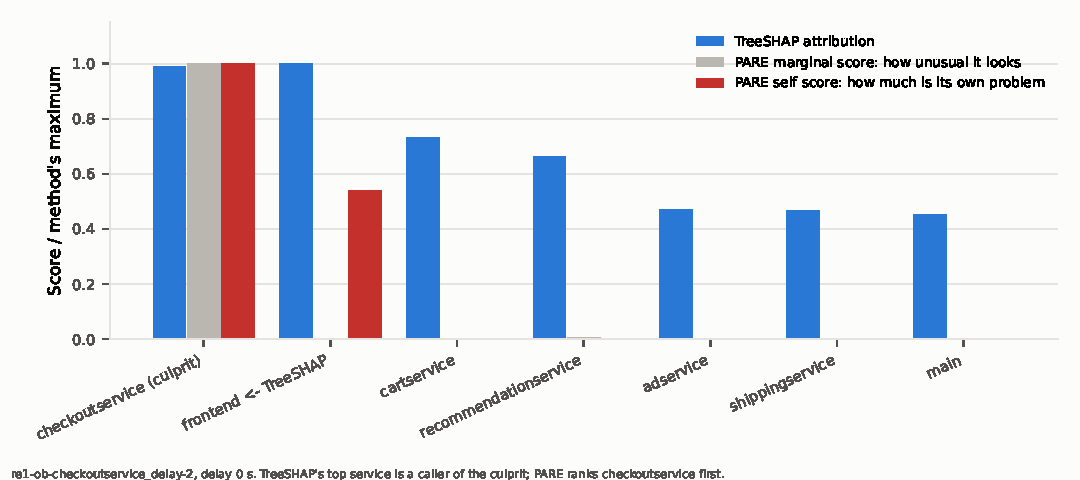
\includegraphics[width=\columnwidth]{figures/fig1_motivating_example.pdf}
\caption{RE1 case \texttt{checkoutservice\_delay-2}: TreeSHAP attribution and PARE
marginal and self scores per service, each scaled to the method's maximum. The case
was selected by a fixed rule: the first case in which TreeSHAP blames a caller and
PARE ranks the culprit first with its highest self score.}
\label{fig:example}
\end{figure}

Figure~\ref{fig:example} shows one case. A delay is injected into
\texttt{checkoutservice}. TreeSHAP spreads attribution over most services and ranks
\texttt{frontend}, a caller of the culprit, first; PARE's scores concentrate on the
culprit.

\subsection{E2: Root-Cause Accuracy}
% Generated by experiments/make_paper_results.py. Do not edit by hand.
\begin{table*}[t]
\centering
\caption{E2/E3: root-cause accuracy with an on-time alarm (0\,s) and a late one (120\,s). Symptom: share of wrong answers that blame a caller of the culprit (lower is better).}
\label{tab:e2}
\footnotesize
\setlength{\tabcolsep}{3pt}
\begin{tabular}{lrrrrrr}
\toprule
& \multicolumn{3}{c}{Delay 0\,s} & \multicolumn{2}{c}{Delay 120\,s} & RE2 \\ \cmidrule(lr){2-4}\cmidrule(lr){5-6}
Method & AC@1 & Avg@5 & Symptom & AC@1 & Avg@5 & AC@1 \\
\midrule
\multicolumn{7}{l}{\textit{RE1 Online Boutique + Sock Shop (250 cases)}} \\
PARE & 0.804 & 0.882 & 0.327 & 0.864 & 0.931 & 0.922 \\
PARE w/o residual & 0.796 & 0.886 & 0.412 & 0.856 & 0.934 & 0.911 \\
PARE w/o change point & 0.888 & 0.945 & 0.607 & 0.860 & 0.926 & 0.922 \\
PARE-LGBM & 0.812 & 0.878 & 0.298 & 0.868 & 0.930 & 0.911 \\
Robust $n$-sigma & 0.852 & 0.948 & 0.649 & 0.836 & 0.942 & 0.922 \\
IForest+TreeSHAP & 0.656 & 0.858 & 0.651 & 0.612 & 0.838 & 0.533 \\
\midrule
\multicolumn{7}{l}{\textit{RE1 Online Boutique (125 cases), alarm time only}} \\
PARE & 0.704 & 0.795 & 0.189 & 0.792 & 0.888 & -- \\
Robust $n$-sigma & 0.744 & 0.885 & 0.219 & 0.832 & 0.923 & -- \\
NSigma~\cite{pham2025rcaeval} & 0.728 & 0.882 & 0.176 & 0.024 & 0.234 & -- \\
BARO~\cite{pham2024baro} & 0.720 & 0.878 & 0.286 & 0.640 & 0.808 & -- \\
CIRCA~\cite{li2022circa} & 0.496 & 0.710 & 0.256 & 0.072 & 0.213 & -- \\
$\varepsilon$-Diagnosis~\cite{shan2019ediagnosis} & 0.056 & 0.202 & 0.136 & 0.064 & 0.184 & -- \\
PC-PageRank~\cite{pham2025rcaeval} & 0.112 & 0.262 & 0.187 & 0.112 & 0.262 & -- \\
\bottomrule
\end{tabular}
\end{table*}


Table~\ref{tab:e2} reports accuracy. On the 250 RE1 cases with a call graph, the
robust $n$-sigma ranker is the most accurate at $d=0$ (AC@1 0.852) and PARE reaches
0.804, but PARE's wrong answers blame a caller far less often: $\mathrm{SR}=0.327$
against 0.649 for $n$-sigma and 0.651 for TreeSHAP. The ablations locate the
effect. Without the residual, AC@1 is almost unchanged (0.796) but SR rises to
0.412, so the residual is what moves wrong answers away from callers. Without the
change point, AC@1 rises to 0.888 at $d=0$: with an on-time alarm there is little to
re-anchor, and an imprecise split can move the window off the fault. Replacing
ridge with LightGBM changes little. On RE2, PARE, $n$-sigma and PARE without change
point tie at 0.922, against 0.533 for TreeSHAP. The strength of a simple robust
ranker agrees with recent evidence that rule-based methods are competitive on
public RCA benchmarks~\cite{fang2026rethinking}; it is also why we report where
wrong answers point, which accuracy alone does not reveal.

Paired tests on the 250 cases show that $n$-sigma ranks better than PARE at $d=0$
($p=0.004$ after Holm correction) with a negligible effect (Cliff's
$\delta=-0.06$); from $d=30$\,s on, the difference is not significant. PARE ranks
significantly better than TreeSHAP at 30, 60 and 120\,s ($p<10^{-5}$,
$\delta=0.22$--$0.24$); at $d=0$ the difference does not survive correction
($p=0.064$).

\noindent\textit{Finding 2: PARE trades a small loss in top-1 accuracy
(significant, but with negligible effect size) for half the symptom blame of the
strongest baseline.}

\subsection{E3: Late Alarms}
\begin{figure}[t]
\centering
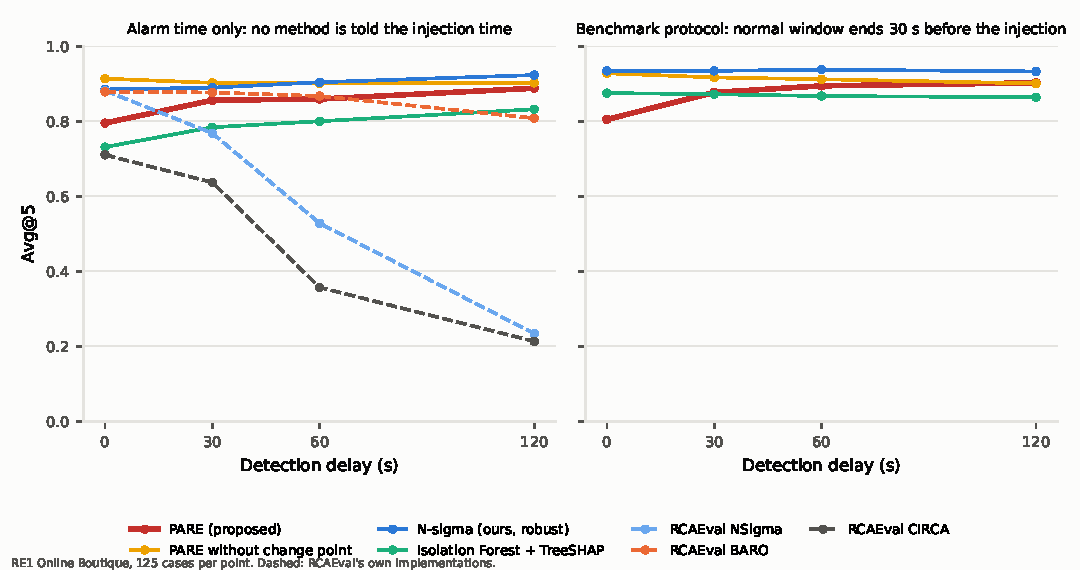
\includegraphics[width=\columnwidth]{figures/fig2_avg5_vs_delay.pdf}
\caption{Avg@5 against detection delay on RE1 Online Boutique (125 cases per
point). (a) Alarm-only protocol, in which no method is told the injection time;
dashed lines are RCAEval's implementations. (b) Benchmark protocol, our methods
only.}
\label{fig:delay}
\end{figure}

Figure~\ref{fig:delay} and the 120\,s columns of Table~\ref{tab:e2} show the effect
of a late alarm. Under the alarm-only protocol, RCAEval's NSigma falls from AC@1
0.728 at $d=0$ to 0.024 at $d=120$\,s, and CIRCA from 0.496 to 0.072; BARO, which
has its own change-point step, holds better (0.640). PARE reaches 0.792 and our
robust $n$-sigma 0.832. No method knows the fault time here, so the difference lies
in how the reference period is chosen: RCAEval's implementations treat everything
before the alarm as normal, which places part of the fault inside the reference
data when the alarm is late. Ending the normal window well before the alarm and
scoring the window by its median \eqref{eq:marginal} avoids this. Under the
benchmark protocol PARE's AC@1 rises with delay, from 0.804 to 0.864 on the 250-case
pool, and passes $n$-sigma at 120\,s (0.836).

\noindent\textit{Finding 3: several published RCA baselines collapse when the alarm
is two minutes late; robust windowed scoring does not.}

\subsection{E4: Sensitivity to the Call Graph}
% Generated by experiments/make_paper_results.py. Do not edit by hand.
\begin{table}[t]
\centering
\caption{E4: PARE on RE2-OB given different call graphs (scored against the true graph).}
\label{tab:e4}
\footnotesize
\setlength{\tabcolsep}{3pt}
\begin{tabular}{lrrr}
\toprule
Graph given to PARE & AC@1 & Avg@5 & Symptom \\
\midrule
Architecture file & 0.922 & 0.969 & 0.286 \\
From traces & 0.922 & 0.967 & 0.286 \\
Correlation-inferred & 0.911 & 0.956 & 0.375 \\
No graph & 0.911 & 0.971 & 0.375 \\
\bottomrule
\end{tabular}
\end{table}

Table~\ref{tab:e4} gives PARE on RE2 with four graphs, always scored against the
manifest graph. The graph read from traces performs exactly like the manifest graph
(AC@1 0.922, $\mathrm{SR}=0.286$), although it lacks four services that emit no
spans. A graph inferred from metric correlations, or no graph, lowers AC@1 slightly
(0.911) and raises SR to 0.375. The graph mainly decides \emph{which} wrong answers
PARE gives, not how many.

\subsection{E5: Faithfulness, Compactness and Stability}
% Generated by experiments/make_paper_results.py. Do not edit by hand.
\begin{table}[t]
\centering
\caption{E5: deletion area (lower is more faithful; random order 0.947), compactness (indicators holding 80\% of the score) and stability under $\pm$10\,s alarm shifts.}
\label{tab:e5}
\footnotesize
\setlength{\tabcolsep}{3pt}
\begin{tabular}{lrrrr}
\toprule
Method & Deletion & Compact. & Jaccard@5 & Kendall $\tau$ \\
\midrule
PARE & 0.542 & 5 & 0.935 & 0.923 \\
PARE w/o residual & 0.406 & 3 & 0.929 & 0.921 \\
Robust $n$-sigma & 0.417 & 2.5 & 0.955 & 0.953 \\
IForest+TreeSHAP & 0.599 & 27 & 0.916 & 0.961 \\
PCA reconstruction & 0.591 & 5 & 0.973 & 0.985 \\
ECDF tail & 0.687 & 18 & 0.935 & 0.947 \\
\bottomrule
\end{tabular}
\end{table}

For the deletion test, the system anomaly score is the mean over the window of the
largest robust $z$-score across metrics; the top $k$ metrics of a method's ranking
are reset to their normal medians for $k=0,\dots,10$, and the area under the
normalised curve is reported (lower is more faithful). Table~\ref{tab:e5}
shows that every method removes the anomaly much faster than a random metric order
(0.41--0.69 against 0.947); PARE beats the random order in 80\% of cases. Marginal
rankers score best ($n$-sigma 0.417, PARE without residual 0.406, PARE 0.542), as
expected: the test rewards removing the loudest metrics first, whereas PARE
deliberately ranks a quieter, unexplained metric above a louder inherited one. The
test should therefore be read alongside accuracy. PARE's explanations are compact
(a median of five metrics carry 80\% of its positive score, against 27 for
TreeSHAP) and stable when the alarm moves by $\pm$10\,s (top-5 Jaccard 0.935,
Kendall $\tau=0.923$).

\subsection{E6: When Does PARE Help?}
\begin{figure}[t]
\centering
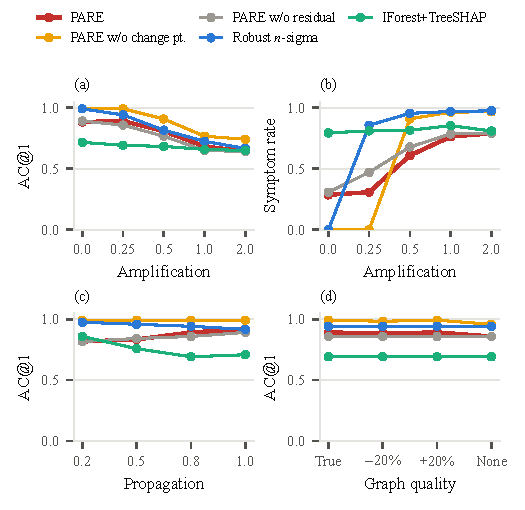
\includegraphics[width=\columnwidth]{figures/fig6_e6_synthetic.pdf}
\caption{Controlled synthetic study, one factor varied at a time (30 seeds
$\times$ 4 fault types per point): AC@1 (a) and symptom rate (b) against
amplification, and AC@1 against propagation strength (c) and graph quality (d). At
low amplification the robust methods make almost no wrong answers, so their symptom
rate there rests on very few cases.}
\label{fig:e6}
\end{figure}

On synthetic systems the cause and the propagation are known exactly. From a base
of ten services, propagation 0.8, amplification 0.25 and the true graph, one factor
is varied at a time (Fig.~\ref{fig:e6}). Under purely linear propagation a caller
can never look worse than its callee, and the robust methods find the culprit
(AC@1 0.992). The trap appears with \emph{amplification}, when a caller degrades
more than proportionally once its callee is slow. As amplification grows from 0.25
to 2.0, PARE without the change-point step stays ahead of $n$-sigma at every level
(0.992, 0.908, 0.767, 0.742 against 0.942, 0.817, 0.725, 0.667). At amplification
0.25 the residual lowers SR from 0.471 (without residual) to 0.308, against 0.857 for
$n$-sigma and 0.811 for TreeSHAP. Graph errors cost little: with 20\% of edges
removed or 20\% wrong edges added, AC@1 stays at 0.983--0.992, and at 0.958 with no
graph. TreeSHAP degrades with system size (0.775 with five services, 0.408 with
forty). As on RE1, the change-point step lowers accuracy (0.892 against 0.992 at the
base setting) and narrows the gap only with a 60\,s delay (0.975 against 1.000).

\noindent\textit{Finding 4: propagation-aware scoring helps exactly where symptoms
are amplified, and tolerates substantial errors in the call graph.}

\section{Discussion and Threats to Validity}

\subsubsection{Which components matter}
Three components carry the gains: robust windowed scoring, which makes our methods
insensitive to late alarms; the residual, which lowers the symptom rate on real and
synthetic data; and the graph walk. The change-point step did not pay off with
prompt alarms on either RE1 or synthetic data, and caught up only when the alarm was
late. We report PARE as designed and recommend disabling re-anchoring when alarms
are known to be prompt.

\subsubsection{Limits of the residual}
On RE1 the residual changes the symptom rate more than the accuracy. Inspecting the
cases where TreeSHAP blames a caller and PARE is right shows why: the ridge model
\eqref{eq:ridge}, fitted on the narrow normal range, extrapolates imperfectly when a
callee moves far outside it, so callers can receive large residuals. PARE still
ranks the culprit first in these cases because the walk \eqref{eq:walk} moves from
the caller to its abnormal callee. Models that extrapolate more conservatively are
a natural next step; tree ensembles are unsuitable because they cannot extrapolate.

\subsubsection{Construct validity}
Disk, delay and loss faults have no metric of their own, so they are excluded from
ExpAC. The symptom rate needs a call graph, which Train Ticket lacks in RE1; its
cases count only toward accuracy.

\subsubsection{External validity}
RE1 and RE2 come from three demonstration applications with injected faults. Real
incidents can be gradual, overlapping or caused by configuration changes. RCAEval's
methods were run as published; their late-alarm behaviour reflects how those
implementations define the normal period, not every possible variant.

\subsubsection{Internal validity}
Every number in this paper is generated by scripts from saved results, with fixed
seeds and saved configurations. One design change was made after a first run on
RE1: the change-point step originally chose the metrics to search using data before
the alarm only, which fails when the alarm is on time; the corrected version is
reported.

\section{Implementation}
PARE runs as a Python library behind a small REST service. A Java Spring Boot
backend manages cases, calls the engine, falls back to a Java $n$-sigma ranker when
the engine is unavailable, and renders results as plain-language explanations. A
React interface shows the call graph with roles, marginal against self scores, and
a replay mode in which an online detector with a conformal threshold watches
arriving metrics and triggers an explanation when it fires. On 20 RE1 cases the
Java benchmark path and the Python experiments return identical rankings.

\section{Conclusion}
Attribution-based explanations of anomaly detectors often point at services that
only suffer from a fault elsewhere, and they rarely name the faulty metric. PARE,
which uses the call graph to subtract what a service inherits from its callees,
halves this symptom error on real benchmark failures, keeps working when the alarm
is late, and costs a small amount of top-1 accuracy (negligible effect size)
against a strong robust baseline. We recommend that RCA evaluations report where wrong answers
point, not only how many answers are right.

\bibliographystyle{IEEEtran}
\bibliography{references}

\end{document}
